\documentclass[a4paper,11pt]{article}
\usepackage{amsmath}
\usepackage{graphicx}
\usepackage{caption}
\usepackage{amssymb}
\usepackage{verbatim}
\usepackage{hyperref}
\usepackage{listings}
\usepackage{float}
\usepackage[thinc]{esdiff}
\usepackage{euscript}
\usepackage{subcaption}
\usepackage{enumitem}
\usepackage{commath}
\setlength{\parindent}{0em}
\newcommand*{\field}[1]{\mathbb{#1}}%
\usepackage{amsthm}
\newtheorem{claim}{Claim}
\captionsetup{labelformat=empty}
\usepackage[nottoc]{tocbibind}
\usepackage{adjustbox}



\begin{document}
\lstset{language = Matlab}
\begin{titlepage} % Suppresses displaying the page number on the title page and the subsequent page counts as page 1
	
	\center % Centre everything on the page
	
	\vspace*{3cm}

	\textsc{Mathematical Tripos, Part II}\\
	\textsc{Computational project}
	\begin{center}
      {\huge\bfseries Boundary Layer Flow\\[0.4cm]
}     \end{center}
	
	\vfill
	\vfill\vfill\vfill\vfill
	\includegraphics*[width = 2.675cm, height = 3.1cm]{coat.png}
	\vfill
    \textsc{University of Cambridge}
	
	\vspace*{\fill}
	\vfill
	{\large\today} 
	\vfill
	
\end{titlepage}
\setcounter{tocdepth}{3}
\tableofcontents

\newpage
\section{Analysis}
\subsection{Question 1}
From the material we have:
\begin{equation*} \label{1.1}
m(f')^{2} - \frac{1}{2}\left(m+1\right)ff'' = m+f''' \tag{1.1}\\
\end{equation*}
With boundary conditions: \begin{equation} \label{1.2}
f' = f = 0\ on\ \eta = 0,\quad f' \to sgnA\ as\ \eta \to \infty . \tag{1.2}
\end{equation}
where $f = f(\eta),\ \eta = y/\delta(x), \ A>0.$\\
When $\eta \to \infty$, we need to check if $f' \sim 1$ in each case.
\begin{enumerate}[label = (\roman*)]
     \item \textbf{algebraic convergence :}\\ \label{i}
     $$f' \sim 1 + B\eta^{-k}  \to 1,\quad as\ \eta \to \infty$$ 

      \item \textbf{exponential convergence :}\\ \label{ii}
      $$f' \sim 1-(\xi+\eta_{0}) \sigma'(\xi) e^{-\sigma(\xi)}  \to 1, \quad as\ \xi \to \infty$$
      where
      $$\sigma'(\xi) = k\xi +k'+k''\xi^{-1} +O(\xi^{-2})$$
      $$\sigma(\xi) = (k/2) \xi^{2} +k' \xi +k'' \log{\xi} + O(\xi^{-1})$$
     So 
     $$f' \sim 1-\xi^{k''}(k\xi^2 + (k'+k\eta_{0})\xi +k''+k'\eta_{0} )e^{-(k/2) \xi^{2} +k' \xi}$$

    \item \textbf{algebraic divergence :}\\ 
    $$f' \sim B(1+k)\eta^{k} \to \infty \quad as\ \eta \to \infty $$ So this case is not possible.
    \item \textbf{exponential divergence :}\\
    $$f' \sim Bke^{k\eta} \to \infty \quad as\ \eta \to \infty$$, so again it is not possible.
    
    \item \textbf{a finite-distant singularity :}\\
    $$f' \sim  B(\eta-\eta_{0})^{-2} \to 0  \quad as\ \eta \to \infty$$, and thus can be incorporated in the asymptotic behaviour alongside \ref{i} or \ref{ii}, but cannot be an asymptotic behaviour of f alone.
\end{enumerate}


    \begin{enumerate}
       \item[(a)]   
           \begin{enumerate}      
           \item[\ref{i}] 
        By means of an asymptotic series solution: 
       $$ f = \sum_{n = -1}^{\infty} a_{n} \eta^{-n}$$ 
       and substitute into \ref{1.1}. By solving for coefficients we can determine B and k without use of conditions at $\eta = 0$. 
           \item[\ref{ii}] 
       f has an asymptotic expansion:
       $$ f = \sum_{n = 0}^{\infty} a_{n} \xi^{-n}e^{-(k/2)\xi^2+k'\xi}$$ 
       and substitute into \ref{1.1}. By solving for coefficients we can determine k, k' and k'' without use of conditions at $\eta = 0$. However, we need them for $\eta_{0}$.
         \end{enumerate}
        \item[(b)]

      For a simplification of \ref{1.1}, we scale  the boundary layer thickness $$\delta = \left(\frac{2\nu x}{(1+m)\abs{U_{e}(x)}}\right)^{\frac{1}{2}}$$ and it becomes \begin{equation} \label{1.3}      
             f''' + ff''+\beta(1-f'^2) = 0,\quad \beta = 2m/(m+1) \tag{1.3}
      \end{equation} with \ref{1.2}.
      Consider $f_{0}$ a 'standard solution' of the equation \ref{1.3} which satisfies \ref{1.2}. Then the perturbed solution is of the form 
      $$f = f_{0}+ \epsilon f_{1} + O(\epsilon^2).$$ Substitute the perturbed solution into \ref{1.3}, we have 
      \begin{equation*}
      f_{0}'''+ \beta(1-f_{0}'^2)+f_{0}f_{0}''+\epsilon (f_{1}''' +f_{1}f_{0}'' +
f_{0}f_{1}''-2\beta\epsilon f_{0}'f_{1}')  +O(\epsilon^{2}) = 0 
      \end{equation*} and thus by solving the coefficient of $O(\epsilon)$,  we have
      \begin{equation*}
      f_{1}''' + f_{1}f_{0}'' + f_{0}f_{1}'' -2\beta f_{0}'f_{1}' = 0 
      \end{equation*}
       assume $f_{0}'' $ decreases faster than $f_{1}$ increases, and as a result:
      \begin{equation} \label{1.4}
      \frac{D^{2}f_{1}'}{D\zeta^{2}} +f_{0} \frac{Df_{1}'}{D\zeta}-2\beta f_{1}' = 0 \tag{1.4}
      \end{equation}
    The equation has been studied by Hartree (1937) \cite{hartree_1937}, and he obtained the asymptotic behaviour:
    \begin{equation*}
    f_1 \sim Ae^{-\frac{\zeta^{2}}{2}}\zeta^{-(2\beta +1)} +B\zeta^{2\beta}
    \end{equation*}
     Then it is clear that the asymptotic behaviour of $f$ is 1 plus above, as $f_{0} \to 1$ when  $\zeta \to \infty.$ Simultaneously, we have verified that $f$ demonstrates algebraic or exponential convergence as indicated previously.
     Accordingly, when $\beta > 0$, we must have $B = 0$ to avoid blow-up at infinity. On the other hand, if $\beta < 0,\ i.e.\ -1<m<0$, it is possible to have both A and B non-zero, and $f_{1}$ tends to 0 for any choice of A and B. When A = 0, the convergence is algebraic.
     In conclusion, for case \ref{i} to be possible, we must have $-1<m<0$ and there is no restriction on \ref{ii}.
     \end{enumerate}

\section{Computational}
The programming task is \ref{Progtsk}
\subsection{Question 2}
Substitute m = 0 and S = 1 into \ref{Progtsk}, from the data obtained we can see that
f' converges to 2.0856... after integrating the system over $\eta$. The convergence indicates that as $eta$ increases to infinity, i.e. goes close to the top of the boundary layer, the horizontal velocity component tends to a constant which is greater than that of the mainstream flow. There is a sudden change in velocity gradient at the interface, which corresponds to a tremendous tangential stress. Therefore, this solution is not physical. \\
\ref{table:Q2} shows the integrated solution with $\eta$ from 0 to 10, with an interval of 0.25. 
To deduce a solution f of \ref{1.1} satisfying the asymptotic behaviour at $\eta \to \infty$, we use the substitution $g = af(b\eta)$ suggested in the material and set ab = 2.0856... corrected to 4 significant figures. We then have 
\begin{equation*} 
\frac{1}{2}ff''+\frac{b}{a}f''' = 0
\end{equation*}
So let b = a = $\sqrt{2.0856}$ we have $f' \to 1$ when $\eta \to \infty$. Then the solution is $g/\sqrt{2.0856}$, and $ f''(0) = (2.0856)^{-\frac{3}{2}}$.

\subsection{Question 3}
\begin{figure}[H]
\begin{subfigure}{0.5\textwidth}
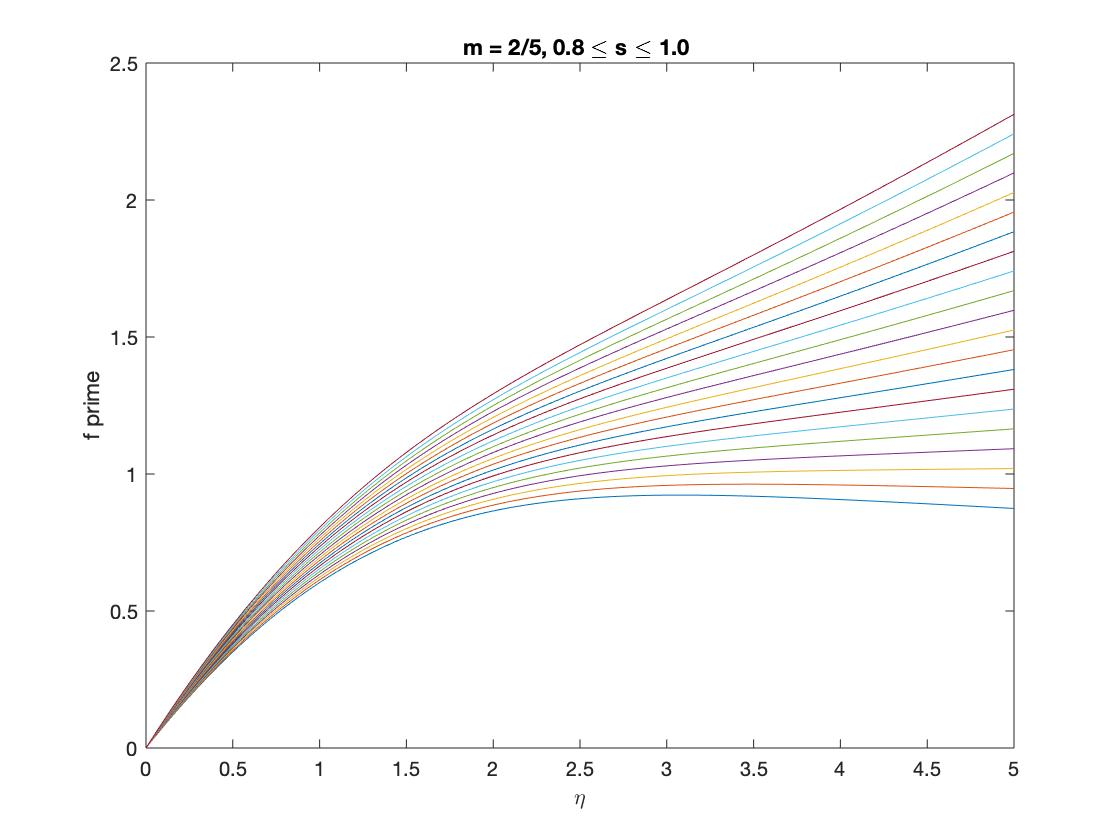
\includegraphics[width = \linewidth, height = 5cm]{Q3(1).jpg}
\caption{Figure 3.1}
\label{Q3(1)}
\end{subfigure}
\begin{subfigure}{0.5\textwidth}
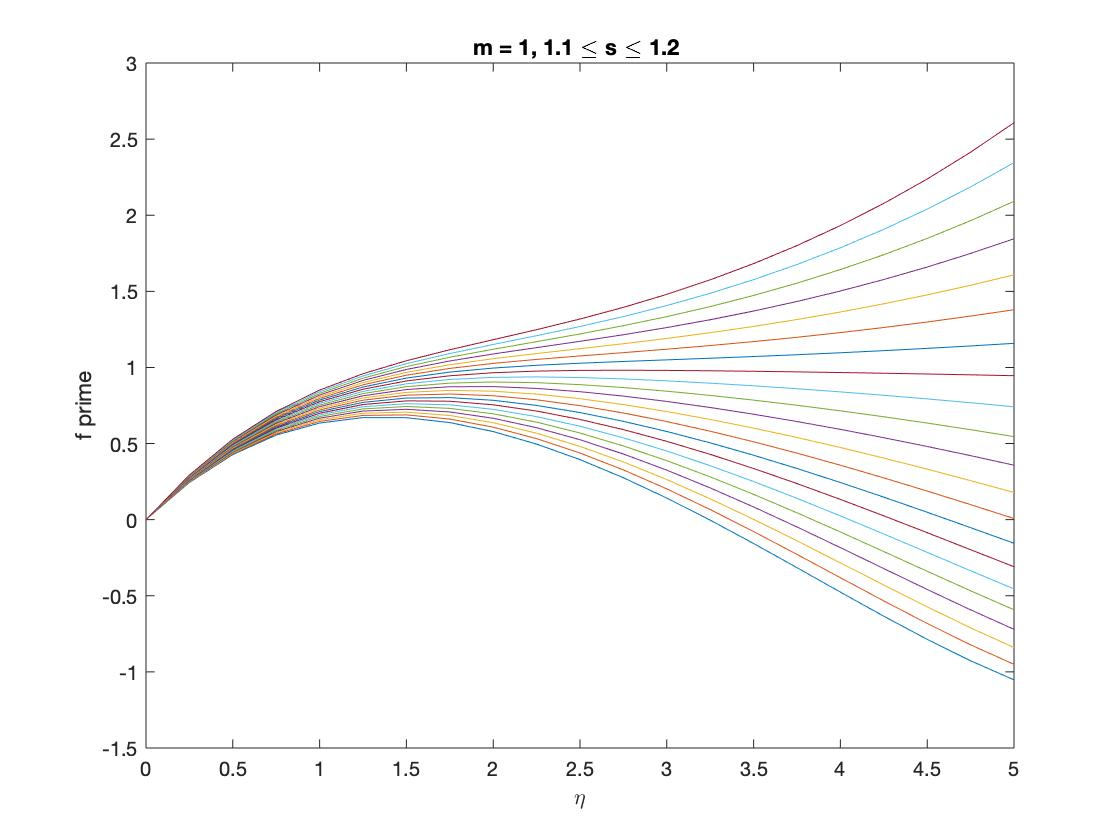
\includegraphics[width = \linewidth, height = 5cm]{Q3(2).jpg}
\caption{Figure 3.2}
\label{Q3(2)}
\end{subfigure}
\caption{Shooting method for m =2/5 and 1}
\label{Q3}
\end{figure}
The programming task is at \ref{S_finder}. From the figures we can see that for in the case where $m = 2/5$, the solution for greater S diverges algebraically, while when $m = 1$ the divergence is exponential. From \ref{S_finder} we can find that $S_{2/5} = 0.8173$, and $s_{1} = 1.1512$. Over $\eta = [0 10]$ we have:
\begin{figure}[H]
\centering
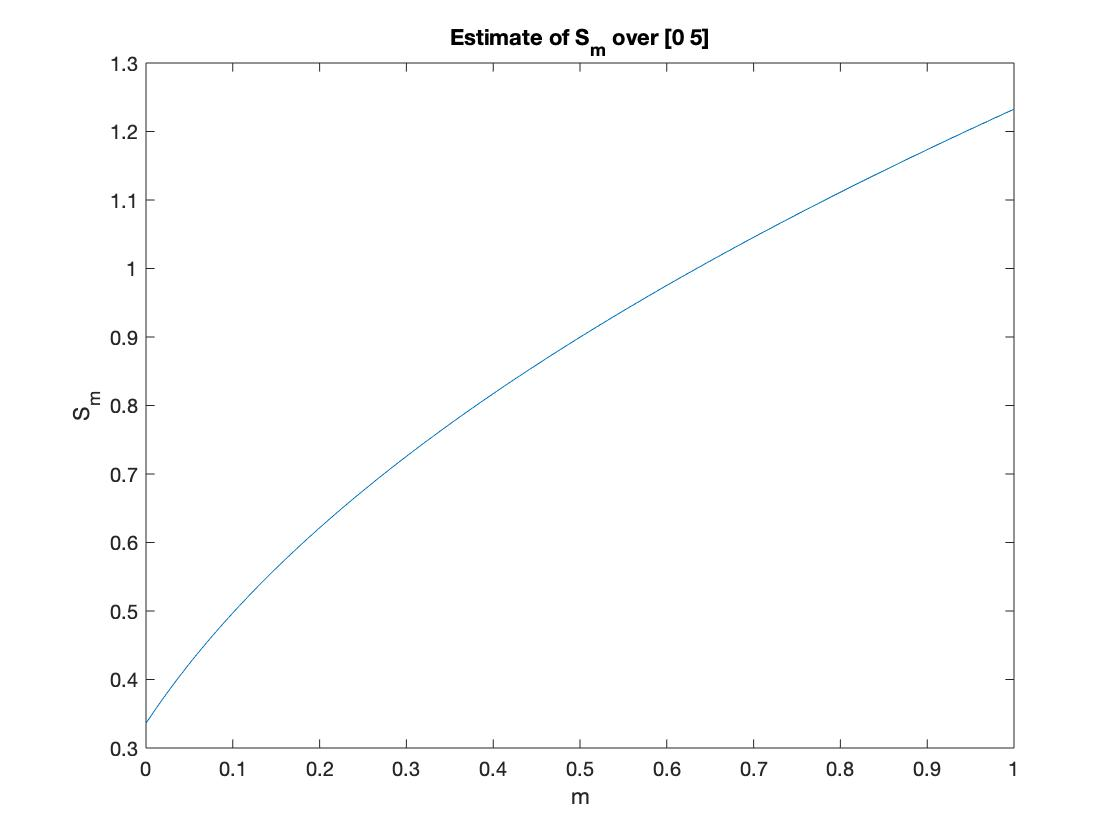
\includegraphics[width= .5\linewidth, height = 5cm]{Q3(3).jpg}
\caption{Plot of estimates of $S_{m}$ against m}
\label{Est.}
\end{figure}
Here I choose $\eta$ up to 5 as this is a value demonstrating a regular asymptotic behaviour of the solution, after integrating further over $\eta$. It is noted that when $\eta$ gets too large the solution diverges considerably. That is because when $\eta$ gets very large, we come out of the boundary layer and the previous equation do not hold.  All values below are accurate to 4 significant figures, by setting the tolerance as 1e-5 in the script. Physically, as m increases, the mainstream flow velocity increases faster as $x \to \infty$. As a result, throughout the boundary layer, the flow increases more rapidly towards the mainstream and thus f''(0) should be larger for a larger m, which also indicates a greater viscous drag due to a steeper velocity gradient at the rigid boundary contact.

\subsection{Question 4}
\begin{figure}[H]
\begin{subfigure}{0.5\textwidth}
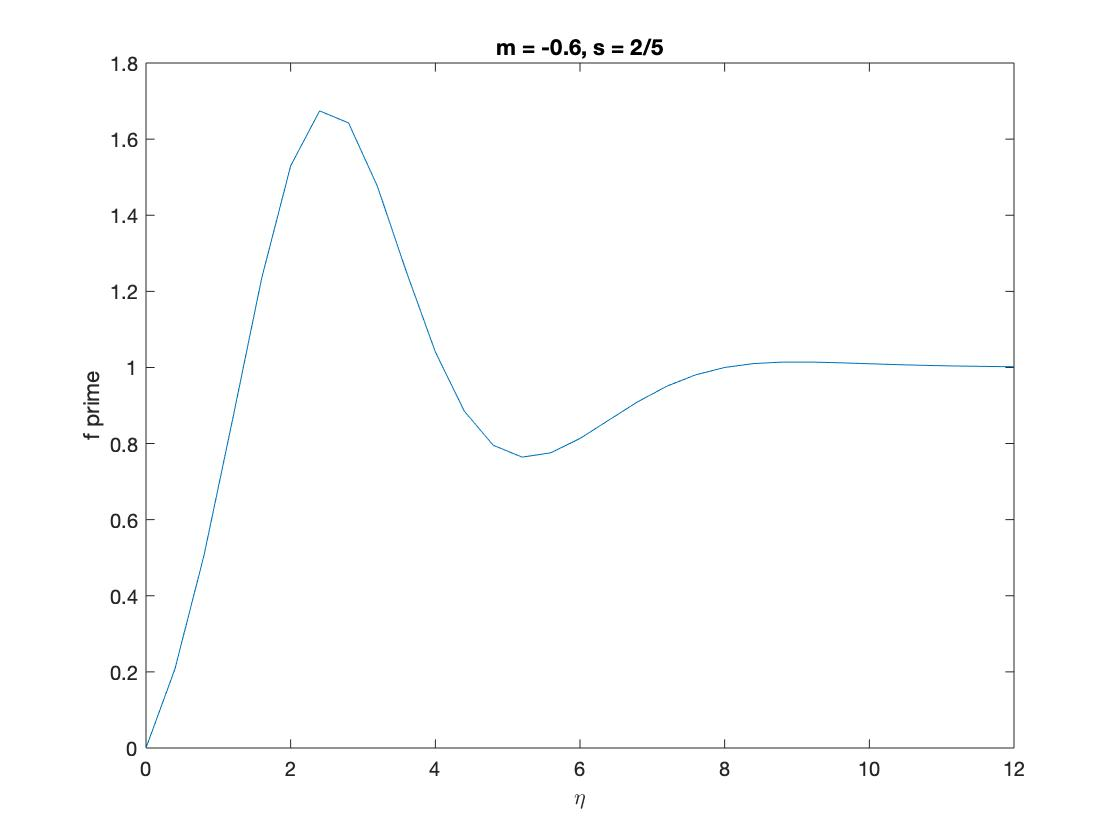
\includegraphics[width = \linewidth, height = 5cm]{Q4(1).jpg}
\caption{Figure 4.1}
\label{Q4(1)}
\end{subfigure}
\begin{subfigure}{0.5\textwidth}
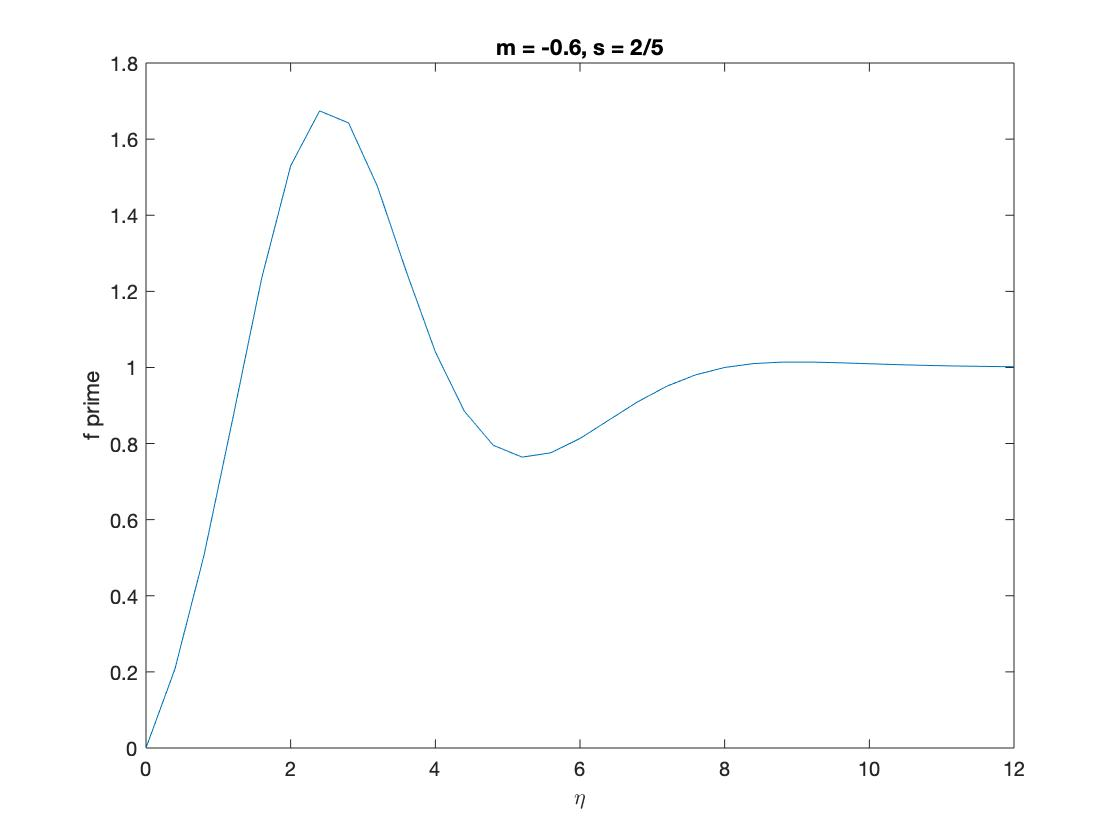
\includegraphics[width = \linewidth, height = 5cm]{Q4(2).jpg}
\caption{Figure 4.2}
\label{Q4(2)}
\end{subfigure}
\begin{subfigure}{0.5\textwidth}
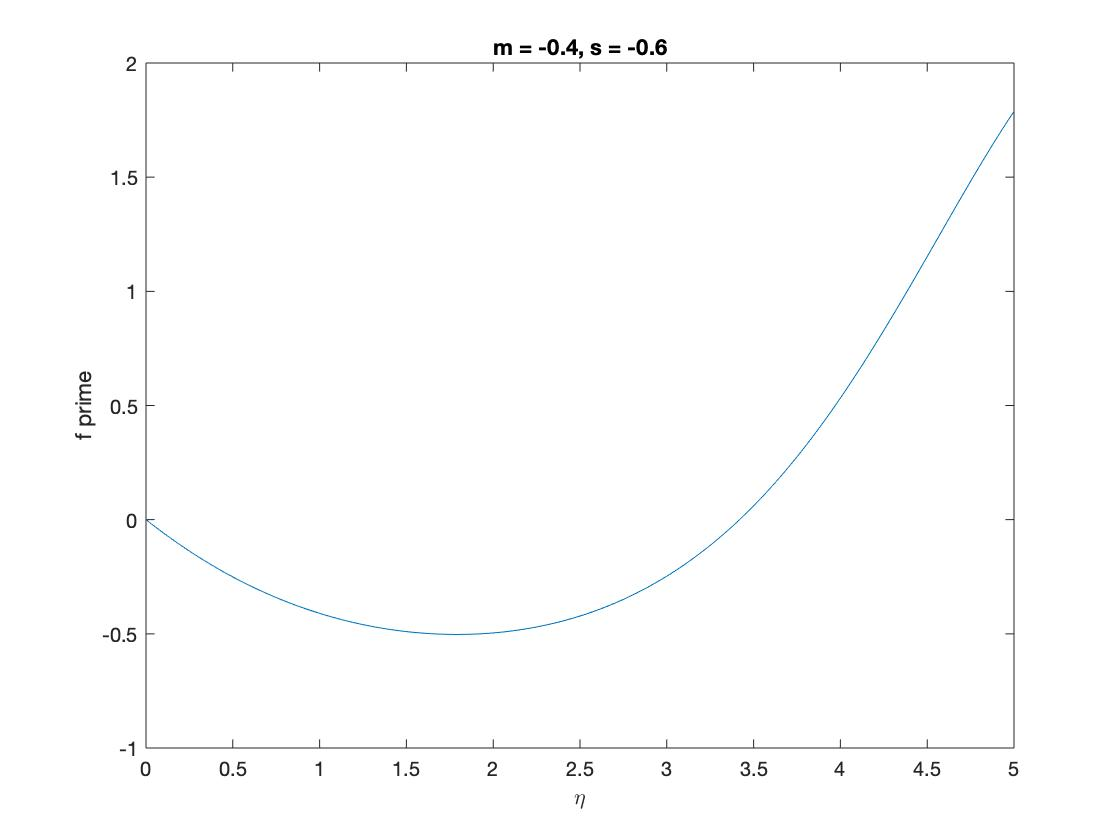
\includegraphics[width = \linewidth, height = 5cm]{Q4(3).jpg}
\caption{Figure 4.3}
\label{Q4(3)}
\end{subfigure}
\begin{subfigure}{0.5\textwidth}
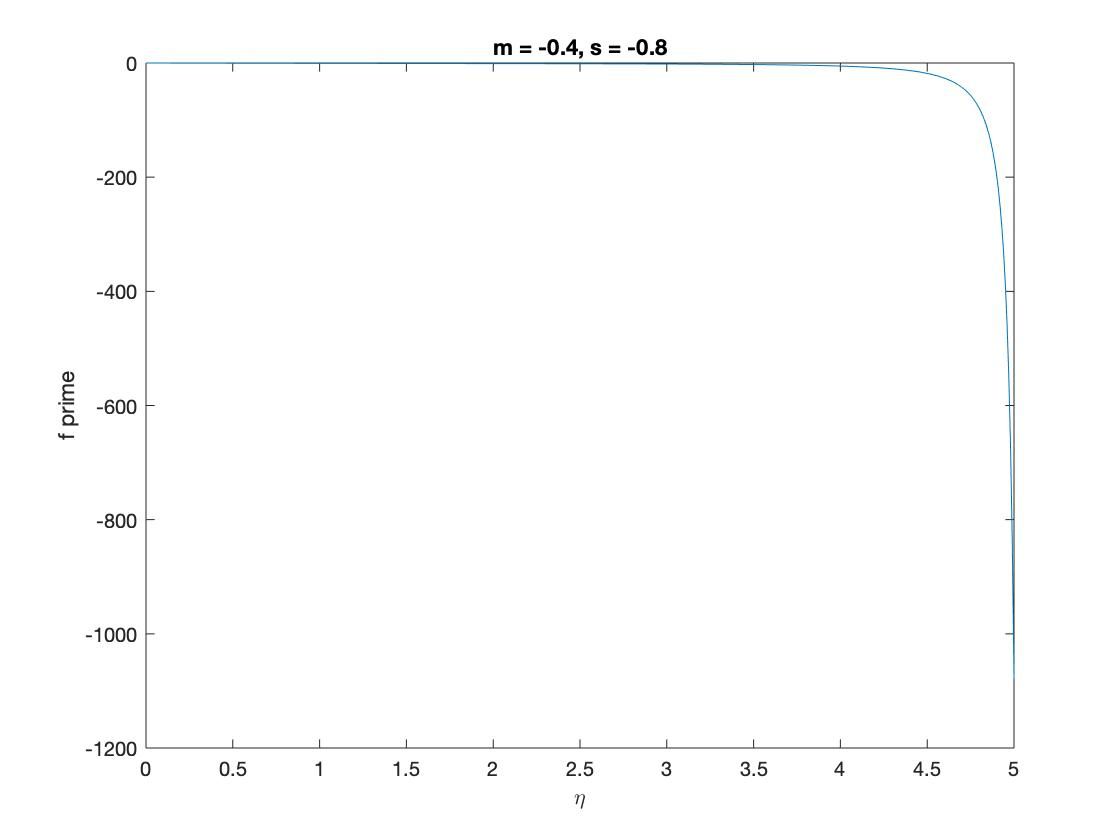
\includegraphics[width = \linewidth, height = 5cm]{Q4(4).jpg}
\caption{Figure 4.4}
\label{Q4(4)}
\end{subfigure}
\begin{subfigure}{0.5\textwidth}
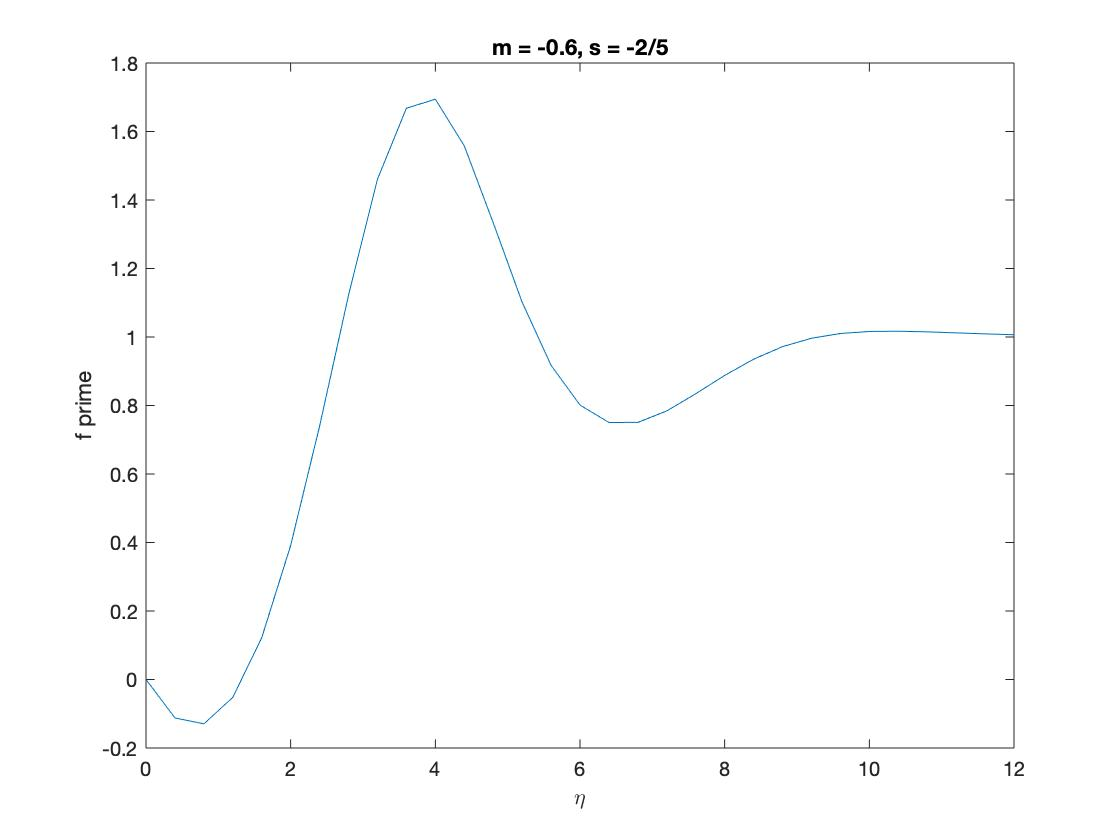
\includegraphics[width = \linewidth, height = 5cm]{Q4(5).jpg}
\caption{Figure 4.5}
\label{Q4(5)}
\end{subfigure}
\begin{subfigure}{0.5\textwidth}
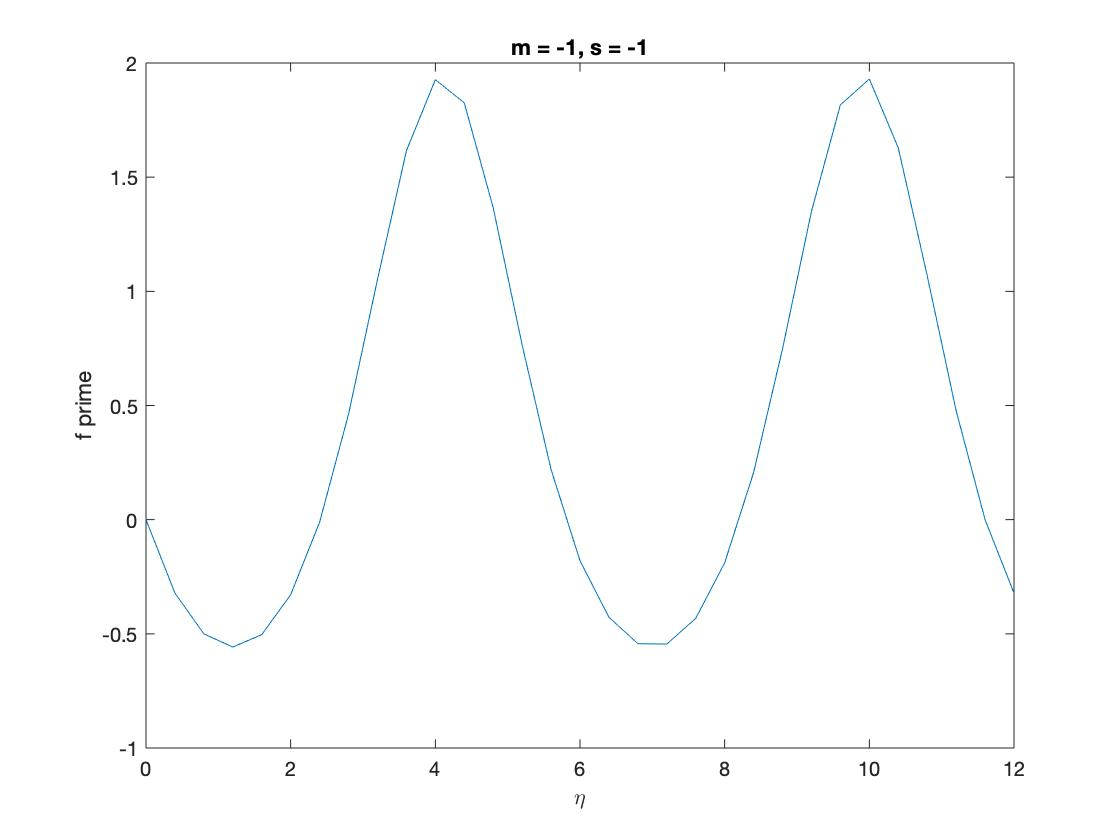
\includegraphics[width = \linewidth, height = 5cm]{Q4(6).jpg}
\caption{Figure 4.6}
\label{Q4(6)}
\end{subfigure}
\label{Q4}
\end{figure}
In \ref{Q4(6)}, the curve diverges algebraically as it wobbles periodically without a decrease in amplitude. In \ref{Q4(1)}, \ref{Q4(2)} and \ref{Q4(5)}, the curves converge quickly over $\eta$, and they converge exponentially as $\eta$ becomes large. In \ref{Q4(3)} and \ref{Q4(4)}, they diverge exponentially. 
The value 

Fix s = 1, for a range of values of m $\in [-1,0]$, the solutions are:
\begin{figure}[H]
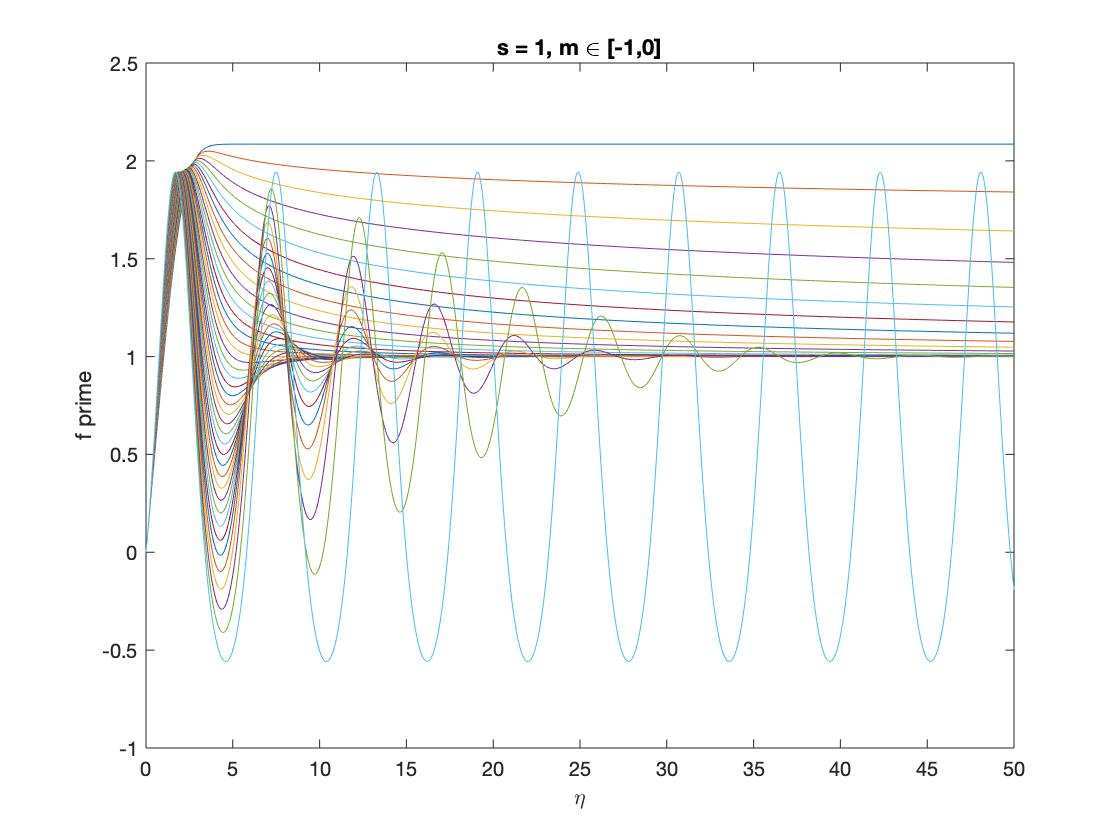
\includegraphics[width = \textwidth, height = 7cm]{Q4(7).jpg}
\end{figure}
If we take a full spectrum of m we have:
\begin{figure}[H]
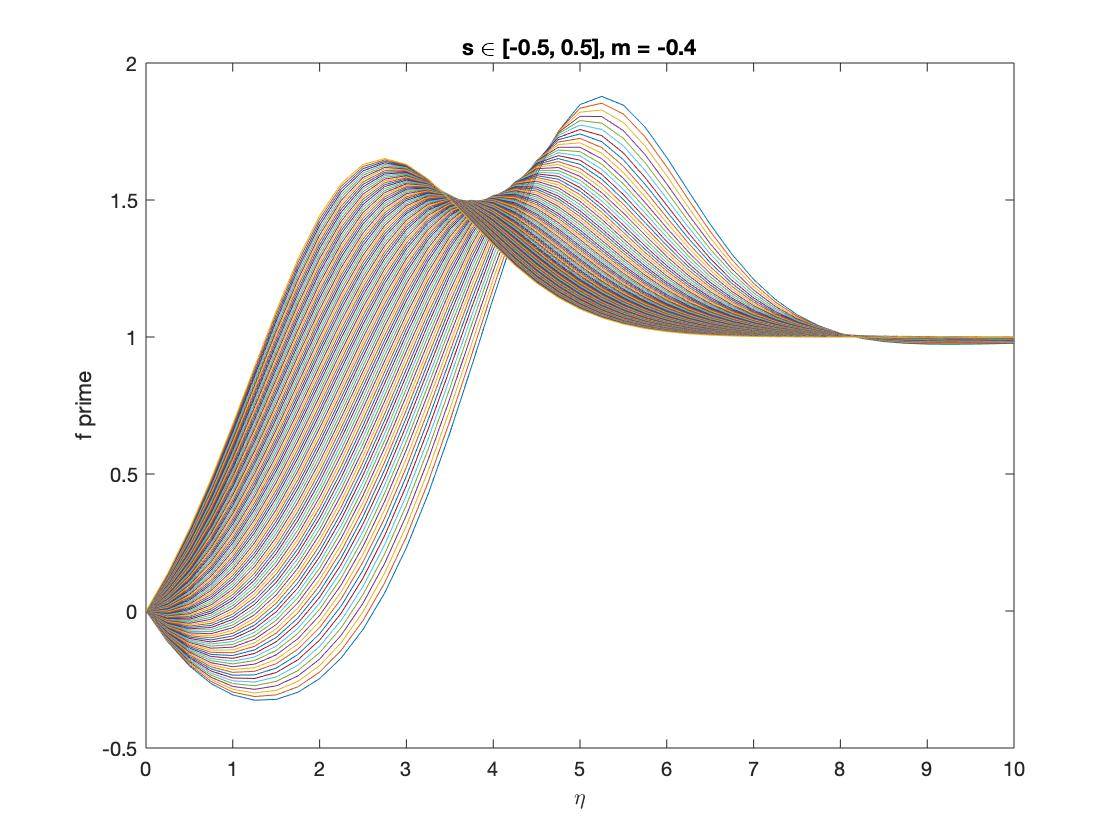
\includegraphics[width = \textwidth, height = 7cm]
{Q4(8).jpg}
\end{figure}
from which we can see one of the branches is a continuation of $m>0$, the other is of a different kind.









\newpage
\section{Codes} 
\subsection{Programming Task 1} \label{Progtsk}
\lstinputlisting{Prog_Task.m} 
\subsection{Programming Task 2} \label{S_finder}
\lstinputlisting{Asympt.m}
\lstinputlisting{S_finder.m}
\lstinputlisting{m_finder.m}
\newpage


\section{Tables}
\begin{table}[H]
\begin{subtable}{.5\linewidth}
\begin{adjustbox}{height =9cm ,center}        
\centering                   
\begin{tabular}{|r|r|r|}     
\hline
f  &f'&f''\\
\hline                       
0.0000 & 0.0000 & 1.0000 \\  
\hline                       
0.0312 & 0.2499 & 0.9987 \\  
\hline                       
0.1249 & 0.4987 & 0.9896 \\  
\hline                       
0.2802 & 0.7435 & 0.9655 \\  
\hline                       
0.4959 & 0.9797 & 0.9203 \\  
\hline                       
0.7689 & 1.2016 & 0.8509 \\  
\hline                       
1.0949 & 1.4033 & 0.7574 \\  
\hline                       
1.4682 & 1.5790 & 0.6457 \\  
\hline                       
1.8820 & 1.7252 & 0.5243 \\  
\hline                       
2.3284 & 1.8410 & 0.4029 \\  
\hline                       
2.8000 & 1.9278 & 0.2921 \\  
\hline                       
3.2901 & 1.9889 & 0.2000 \\  
\hline                       
3.7929 & 2.0293 & 0.1290 \\  
\hline                       
4.3037 & 2.0547 & 0.0778 \\  
\hline                       
4.8194 & 2.0696 & 0.0440 \\  
\hline                       
5.3379 & 2.0778 & 0.0233 \\  
\hline                       
5.8580 & 2.0820 & 0.0116 \\  
\hline                       
6.3788 & 2.0841 & 0.0054 \\  
\hline                       
6.8999 & 2.0850 & 0.0024 \\  
\hline                       
7.4212 & 2.0854 & 0.0010 \\  
\hline                       
7.9426 & 2.0855 & 0.0004 \\  
\hline                       
8.4640 & 2.0856 & 0.0001 \\  
\hline                       
8.9854 & 2.0856 & 0.0000 \\  
\hline                       
9.5068 & 2.0856 & 0.0000 \\  
\hline                       
10.0282 & 2.0856 & 0.0000 \\ 
\hline                       
10.5496 & 2.0856 & 0.0000 \\ 
\hline                       
11.0710 & 2.0856 & 0.0000 \\ 
\hline                       
11.5924 & 2.0856 & 0.0000 \\ 
\hline                       
12.1138 & 2.0856 & -0.0000 \\
\hline                       
12.6352 & 2.0856 & -0.0000 \\
\hline                       
13.1566 & 2.0856 & -0.0000 \\
\hline                       
13.6780 & 2.0856 & -0.0000 \\
\hline                       
14.1994 & 2.0856 & 0.0000 \\ 
\hline                       
14.7208 & 2.0856 & 0.0000 \\ 
\hline                       
15.2422 & 2.0856 & 0.0000 \\ 
\hline                       
15.7636 & 2.0856 & 0.0000 \\ 
\hline                       
16.2850 & 2.0856 & -0.0000 \\
\hline                       
16.8064 & 2.0856 & 0.0000 \\ 
\hline                       
17.3279 & 2.0856 & -0.0000 \\
\hline                       
17.8493 & 2.0856 & -0.0000 \\
\hline                       
18.3707 & 2.0856 & 0.0000 \\ 
\hline                       
\end{tabular}         
\end{adjustbox}       
\caption{Table 1}         
\label{table:Q2}             
\end{subtable}%                 
\begin{subtable}[t]{.5\textwidth} 
\begin{adjustbox}{height =9cm ,center}        
\centering                   
\begin{tabular}{|c|c|}      
\hline 
m& $s_{m}$\\
\hline                   
0.0000 & 0.3362 \\        
\hline                    
0.0250 & 0.3816 \\        
\hline                    
0.0500 & 0.4231 \\        
\hline                    
0.0750 & 0.4614 \\        
\hline                    
0.1000 & 0.4972 \\        
\hline                    
0.1250 & 0.5308 \\        
\hline                    
0.1500 & 0.5625 \\        
\hline                    
0.1750 & 0.5927 \\        
\hline                    
0.2000 & 0.6215 \\        
\hline                    
0.2250 & 0.6490 \\        
\hline                    
0.2500 & 0.6755 \\        
\hline                    
0.2750 & 0.7011 \\        
\hline                    
0.3000 & 0.7258 \\        
\hline                    
0.3250 & 0.7497 \\        
\hline                    
0.3500 & 0.7728 \\        
\hline                    
0.3750 & 0.7954 \\        
\hline                    
0.4000 & 0.8173 \\        
\hline                    
0.4250 & 0.8386 \\        
\hline                    
0.4500 & 0.8595 \\        
\hline                    
0.4750 & 0.8798 \\        
\hline                    
0.5000 & 0.8997 \\        
\hline                    
0.5250 & 0.9192 \\        
\hline                    
0.5500 & 0.9383 \\        
\hline                    
0.5750 & 0.9570 \\        
\hline                    
0.6000 & 0.9753 \\        
\hline                    
0.6250 & 0.9933 \\        
\hline                    
0.6500 & 1.0110 \\        
\hline                    
0.6750 & 1.0284 \\        
\hline                    
0.7000 & 1.0455 \\        
\hline                    
0.7250 & 1.0624 \\        
\hline                    
0.7500 & 1.0789 \\        
\hline                    
0.7750 & 1.0953 \\        
\hline                    
0.8000 & 1.1114 \\        
\hline                    
0.8250 & 1.1272 \\        
\hline                    
0.8500 & 1.1429 \\        
\hline                    
0.8750 & 1.1583 \\        
\hline                    
0.9000 & 1.1735 \\        
\hline                    
0.9250 & 1.1886 \\        
\hline                    
0.9500 & 1.2034 \\        
\hline                    
0.9750 & 1.2181 \\        
\hline                    
1.0000 & 1.2326 \\                  
\hline                    
\end{tabular}        
\end{adjustbox}       
\caption{Table 2}  
\label{table:Q3}
\end{subtable}               
\end{table}

\bibliographystyle{unsrt}
\bibliography{cite}
\end{document}